% simple.tex - A simple article to illustrate document structure.

% Andrew Roberts - June 2003

\documentclass[16pt, article,notitlepage]{article}
\usepackage[spanish]{babel}%Para el español
\usepackage[utf8]{inputenc}


%\usepackage{times}
\usepackage{color}
\usepackage[dvipsnames]{xcolor}
\usepackage{listings}
\usepackage{textcomp}
\usepackage[a4paper, total={6in, 8in}]{geometry}
\usepackage{pdfpages}

\usepackage{verbatim}

\usepackage{amsmath}
\usepackage{courier} %--lisitngs
\usepackage{mathptmx} %-->TimesNewRoman

\usepackage{caption}
\DeclareCaptionFont{white}{\color{white}}
\definecolor{dark-gray}{cmyk}{0,0,0,0.7}
\DeclareCaptionFormat{listing}{\colorbox{dark-gray}{\parbox{\textwidth}{#1#2#3}}}
\captionsetup[lstlisting]{format=listing,labelfont={white,sf},textfont={white,sf}}

\usepackage{graphicx} % Required for including pictures

\usepackage{float} % Allows putting an [H] in \begin{figure} to specify the exact location of the figure
\usepackage{wrapfig} % Allows in-line images such as the example fish picture
\graphicspath{{Imagenes/}} % Specifies the directory where pictures are stored

\usepackage{xcolor}
\definecolor{lbcolor}{rgb}{0.9,0.9,0.9}
\lstset{
backgroundcolor=\color{gray!20!white},
    tabsize=2,
    literate=%
	{á}{{\'{a}}}1
    {é}{{\'{e}}}1
    {í}{{\'{i}}}1
    {ó}{{\'{o}}}1
    {ú}{{\'{u}}}1
    {ñ}{{\~{n}}}1
    {<}{{$<$}}1
    {>}{{$>$}}1,
%   rulecolor=,
    %language=C,
    %language=bash,
    	linewidth=12.2cm,
		belowcaptionskip=0.1\baselineskip,
		xleftmargin=\parindent,        
        %basicstyle=\scriptsize,
        basicstyle=\footnotesize\bfseries\ttfamily\color{black!80!white},
        upquote=true,
        %aboveskip={1.5\baselineskip},
        columns=fixed,
       	showstringspaces=false,
        extendedchars=false,
        breaklines=true,
        prebreak = \raisebox{0ex}[0ex][0ex]{\ensuremath{\hookleftarrow}},
	%frame=lines,
        numbers=left,
        showtabs=false,
        showspaces=false,
        showstringspaces=false,
        identifierstyle=\ttfamily,
        commentstyle=\color{orange!80!black},
        keywordstyle=\bfseries\color[rgb]{0,0,1},
        %commentstyle=\bfseries\color[rgb]{0.026,0.112,0.095},
        %stringstyle=\bfseries\color[rgb]{0.627,0.126,0.941},
        stringstyle=\bfseries\color{green!50!black},
        numberstyle=\ttfamily\color[rgb]{0.205, 0.142, 0.73},
%        \lstdefinestyle{C++}{language=C++,style=numbers}’.
}
\lstdefinelanguage{linux_bash}
{ language=bash,%-->me baso en bash
alsoletter={-},%-->me habilita (-) en medio de los keywords
morekeywords={sudo,nano,apt-get,cd,ls,ln,mkdir,ifconfig,cp,wget,ppa:,add-apt-repository,install,a2ensite,service,curl},
%sensitive=false,
}
\lstdefinelanguage{cisco}
{
alsoletter={-},%-->me habilita (-) en medio de los keywords
keywords={enable,configure,terminal,interface,fastEthernet,ipv6,address,no,shutdown,route,running-config,startup-config,copy,exit,unicast-routing,brief},
%sensitive=false,
}

\renewcommand{\lstlistingname}{Código}
\renewcommand{\familydefault}{\rmdefault}
\pretolerance=2000
\tolerance=3000
\newcommand{\HRule}{\rule{\linewidth}{0.5mm}} % Defines a new command for the horizontal lines, change thickness here
\usepackage{hyperref}
\hypersetup{%
colorlinks=true,
urlcolor=blue,
urlbordercolor=blue,
pdfborderstyle={/S/U/W 1}%
}

\begin{document}

\begin{figure}[H] % Example image
	\center{
\includegraphics[width=0.8\linewidth]{./images/header_unc.png}}
\end{figure}

% Article top matter

\title{%\HRule \\[0.4cm]		
	{ \bfseries{Trabajo Final - Control Remoto de un portón doméstico}}\\[0.4cm]
	%\HRule \\[1.5cm]
} %\LaTeX is a macro for printing the Latex logo
\author{
	\textsc{Tomattis}, Natasha  {\small \texttt{Mat:38.728.783}}\\
	\href{mailto:natitomattis@gmail.com}{natitomattis@gmail.com}\\
	\textsc{Trombotto}, Agustín  {\small \texttt{Mat:39.071.116}}\\
	\href{mailto:gutitrombotto@gmail.com}{gutitrombotto@gmail.com}\\
	\textsc{Aguerreberry}, Matthew  {\small \texttt{Mat:93.739.112}}\\
	\href{mailto:mtaguerreberry@gmail.com}{mtaguerreberry@gmail.com}\\
}
%\affil{Facultad de Ciencias Exáctas, Físicas \& Naturales, Universidad Nacional de Córdoba, Argentina.}

%\date{\today}  %\today is replaced with the current date
%\maketitle
{\let\newpage\relax\maketitle}

\newpage

\maketitle
 
\tableofcontents

\newpage
\section{Introducción}
 
En este informe se desarrolla el modelado, la implementación y la documentación de un sistema de Computación. Un Sistema de computación o también llamado “Cyber Physical System” está constituido tanto por componentes de hardware como por software además de la relación que el mismo tiene con el usuario y con el ambiente que lo rodea. En este caso, se desarrollará un sistema de control de un portón electrico con conexion remota mediante un dispositivo móvil. \\
Para la realización de este proyecto se tendrá en cuenta el standard SYSML para el modelado del problema. El mismo provee un esquema gráfico que facilita el diseño del sistema y a su vez ayuda en la obtención de requerimientos funcionales. \\
El sistema desarrollado tiene un enfoque principalmente al usuario. Por ende se tiene en cuenta el fácil uso y la sencilla implementación teniendo, por este motivo, algunas limitaciones en lo tecnológico.

\section{Marco Teórico}
Se va a desarrollar un controlador para portones automáticos que permite una rápida instalación en un portón automático convencional, controlado desde una aplicacion de celular. \\
La motivación es que los usuarios no tengan riesgos de extraviar los controles de los portones automáticos, lo cual no solo afectaría al usuario en que no podrá ingresar a su garaje sino que también sería una amenaza a su seguridad ya que un control convencional no cuenta con una autenticación de usuario. 
\subsection{Comparación con potenciales competidores}

Se analizó las ofertas en el mercado de productos similares o sustitutos al sistema que se va a desarrollar. En un principio tras un análisis en el mercado local (Argentina) no se obtuvieron resultados de un producto que se encontrara a la venta con estas características.
Por otro lado en un mercado más amplio se obtuvieron dos resultados de productos sustitutos, ambos cumplen la misma funcionalidad pero implementados de diferente manera
\subsubsection{OPEN-SESAME}

Open Sesame Garage Door Opener ofrece una pequeña caja bluetooth y una aplicación para smartphone que controla el portón a través de una conexión bluetooth. El precio de este producto es el de un control regular, incentivando a los clientes de esta forma a reemplazar los controles infrarrojos convencionales.

\begin{figure}[H] 
	\centering
	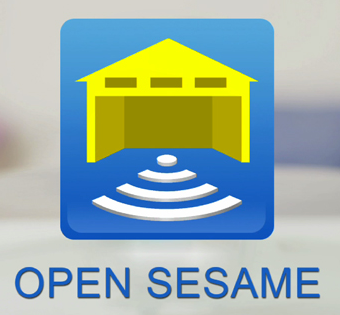
\includegraphics[scale=0.7]{./images/opensesame.png}
	\caption{\textit{ Logo de Gogogate}}
\end{figure}

\href{https://www.mygarageopener.com/}{Pagina web de OPEN-SESAME}



\subsubsection{GOGOGATE}

Es una solución más completa, a diferencia del producto anterior este se comunica con el cliente a través de la red LAN del hogar.  Tiene una aplicación móvil mucho más completa con control de acceso de usuarios, permitiendo el ingreso de diferentes clases de usuarios, un servicio de cámara para monitorear el garage, una sirena que advierte cuando el portón se abre o cierra, sensor de temperatura, entre otros servicios.  Desde el punto de vista de hardware ofrece un dispositivo con cámara y alarma integrada, capacidad para conexión por ethernet o wireless

\begin{figure}[H] 
	\centering
	
\includegraphics[scale=0.7]{./images/gogogate_logo.png}
	\caption{\textit{ Logo de Gogogate}}
\end{figure}

\begin{figure}[H] 
	\centering
	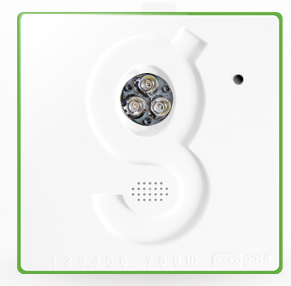
\includegraphics[scale=0.6]{./images/gogogate_disp.png}
	\caption{\textit{ Dispositivo de Gogogate}}
\end{figure}



\href{https://www.gogogate.com/index.html}{Pagina web de Gogogate}

\section{Requerimientos Funcionales}

\subsection{Instalación sencilla}
Actualmente, los portones automáticos manejados por un simple control remoto independiente, dominan el mercado. Para que los usuarios tomen la iniciativa de cambiar de sistema este nuevo sistema debe ser de fácil y rápida instalación, de no ser así, los usuarios no optarán por realizar el cambio ya que implicaría un gran gasto de dinero y tiempo.
Para lograr esto, el hardware utilizado será un simple embebido de bajo costo y gran disponibilidad. 
\subsection{Fácil uso}
La interfaz de usuario debe ser amigable e intuitiva. Tendrá un diseño orientado para dispositivos táctiles. No contendrá muchas opciones de configuración, ya que esto será concentrado en el servidor de control.
\subsection{Seguridad}
Aquí se exige que solamente el usuario autorizado pueda ser capaz de controlar el comportamiento del portón. Para esto, se le solicitará al usuario se registre inicialmente en el sistema. Luego, cuando se desee abrir o cerrar el portón dicho usuario deberá proporcionar un PIN de autenticación extra.
\section{Diseño}
SysMl define tres grupos de diagramas a alto nivel, estructura (modelo estático), comportamiento (modelo dinámico) y requerimientos. Los requerimientos en este caso ya fueron definidos anteriormente, ahora definiremos los bloque restantes: 
\subsection{Modelado a nivel de sistema}
Para este caso se utilizo un diagrama de definición de bloques para mostrar la relación entre los elementos del sistema y los elementos externos que afectaran al comportamiento del sistema.

\begin{figure}[H]
	\centering{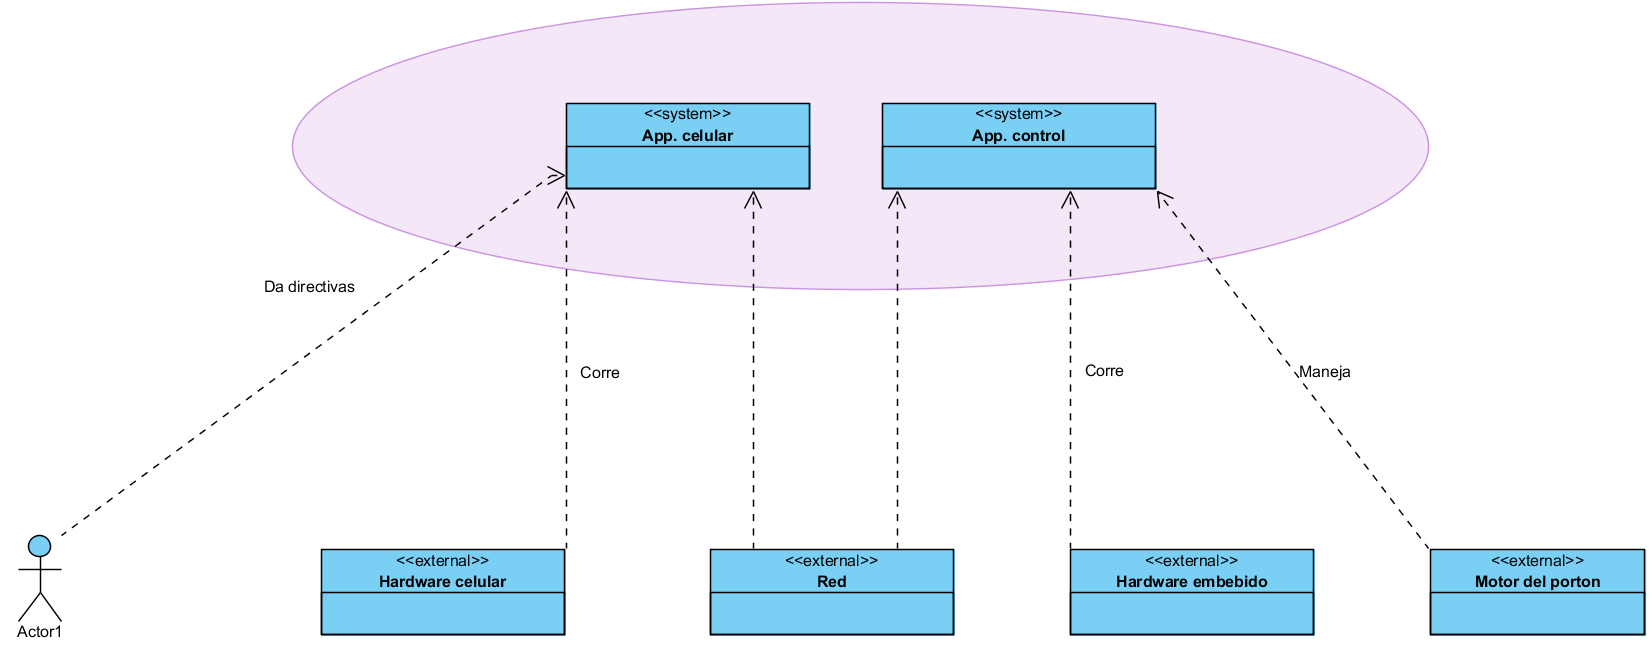
\includegraphics[width=0.8\linewidth]{./images/DiagramaDeEstructura.png}}
	\caption{Diagrama de estructura}
	
\end{figure}
Se puede ver que la zona sombreada son los elementos que son parte del sistema y en el extremo inferior los elementos que afectan en su comportamiento
\\
Una vez definida la relación del sistema con su entorno se definen los bloques internos de las partes de los elementos del sistema en este caso la App Móvil y App Control
\\
\begin{itemize}
	\item App Móvil Es la aplicación que correrá en el dispositivo móvil del cliente, por lo tanto se deberán tener en cuenta las librerías que permitan a la aplicación comunicarse con el entorno
	\begin{figure}[H]
		\centering{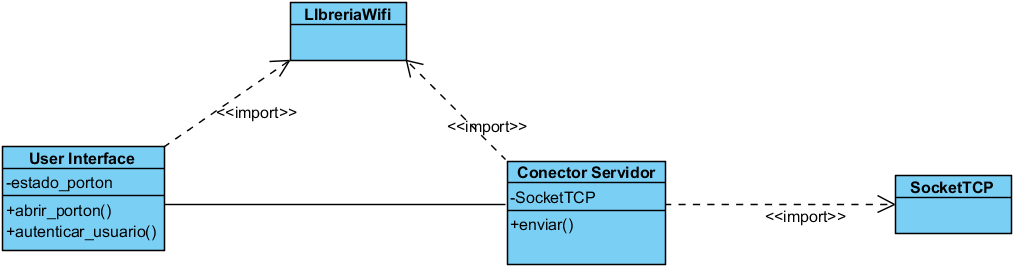
\includegraphics[width=0.8\linewidth]{./images/AppCelular.png}}
		\caption{Diagrama de clases de App Movil}
	\end{figure}
	\item App Control esta aplicación correrá en el hardware embebido, por lo tanto también deberá incluir las librerías de los módulos que utilizará.
	\begin{figure}[H]
		\centering 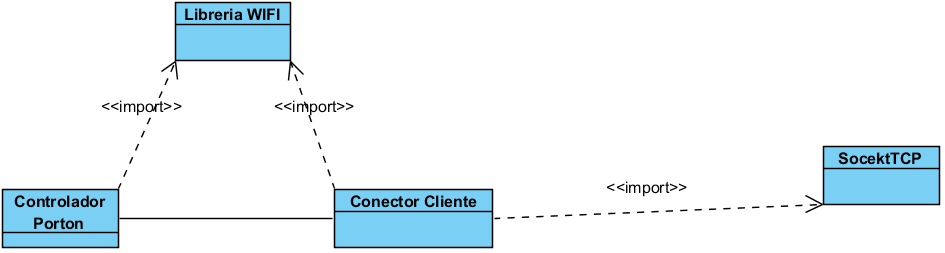
\includegraphics[width=0.8\linewidth]{./images/AppControl.png}
		\caption{Diagrama de clases de App Control}
	\end{figure}
\end{itemize}

\subsection{Comportamiento}
Para comenzar con el análisis de comportamiento se realizo un diagrama de casos de uso que brinda una una descripción a muy alto nivel de las funcionalidades del sistema, respecto al usuario. Dado que el comportamiento del sistema es muy sencillo en este caso solo se analiza un caso de uso.
\begin{figure}[H]
	\centering 
	{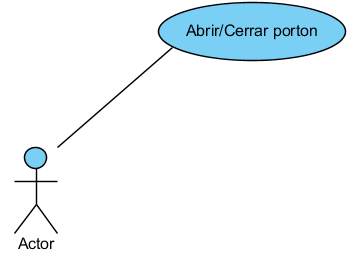
\includegraphics[width=0.3\linewidth]{./images/CasosDeUso.png}}
	\caption{Diagrama de casos de uso}
\end{figure}
Una vez definido el caso de uso, se analizan las acciones que se deben llevar a cabo para cumplir con esa funcionalidad para esto se confecciona diagrama de actividad.
\begin{figure}[H]
	\centering{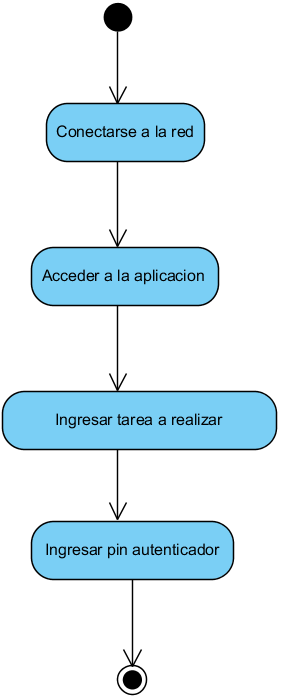
\includegraphics[width=0.3\linewidth]{./images/Actividad.png}}
	\caption{Diagrama de actividad de abrir/cerrar portón}
\end{figure}
Un diagrama de secuencia nos mostrara la interacción entre las diferentes partes del sistema cuando durante el caso de uso abrir/cerrar portón:
\begin{figure}[H]
	\centering{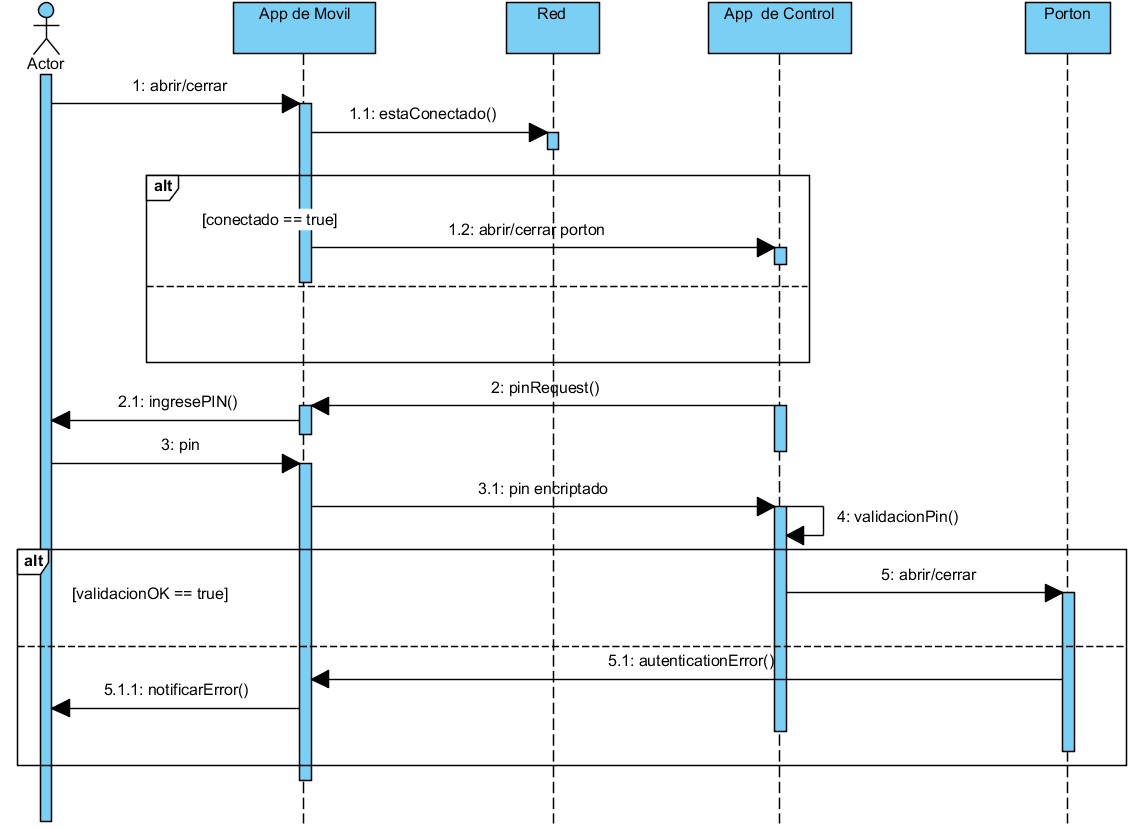
\includegraphics[width=0.8\linewidth]{./images/Secuencia.png}}
	\caption{Diagrama de secuencia abrir/cerrar portón}
\end{figure}

\section{Decisión de diseño}
Luego de la descripción y modelado del sistema se define los recursos puntales que usaremos. Los mismos son los siguientes:

\begin{itemize}
	\item   Hardware Embebido: Raspberry Pi 3; este hardware tiene la capacidad de procesamiento necesaria para soportar los requerimientos del sistema, además de las interfaces necesarias como conectividad WiFi.
	\item App Control: se desarrollará en el lenguaje Python. Python es un lenguaje interpretado que posee gran cantidad de librerías para el manejo de interfaces en la Raspberry Pi. Además es de muy fácil uso y tiene una comunidad grande para enfrentar cualquier dificultad.
	\item   App Celular: se usará Android Studio para crear la aplicación de celular. El mismo brinda un manejo muy fácil para programan, montando en java y con gran cantidad de clases de uso general del dispositivo.
	
\end{itemize}

\section{Bibliografía}



%\begin{figure}[H] % Example image
%	\center{\includegraphics[width=0.8\linewidth]{./mensajesUdpWireshark.png}}
%	\caption{Mensajes UDP analiados en Wireshark}
%	\label{fig:top_en1}
%\end{figure}

\end{document}

